\documentclass{article}

% arXiv preprint style; swap for the target workshop's template on acceptance.
\usepackage[margin=1in]{geometry}
\usepackage{amsmath,amssymb,amsfonts}
\usepackage{booktabs}
\usepackage{graphicx}
\usepackage{microtype}
\usepackage{xcolor}
\usepackage[colorlinks=true,linkcolor=blue!60!black,citecolor=blue!60!black,urlcolor=blue!60!black]{hyperref}
\usepackage[numbers]{natbib}
\usepackage{caption}
\usepackage{tikz}
\usetikzlibrary{positioning}
\captionsetup{font=small,labelfont=bf}

% Nine figures over nine pages: loosen float limits so each stays near its
% section instead of queueing up behind the references.
\renewcommand{\topfraction}{0.92}
\renewcommand{\textfraction}{0.06}
\renewcommand{\floatpagefraction}{0.85}
\setcounter{topnumber}{3}
\setcounter{totalnumber}{4}

\newcommand{\lace}{\textsc{LACE}}
\newcommand{\sg}{\mathrm{sg}}
\newcommand{\Estud}{E_{\theta}}
\newcommand{\Efroz}{E_{\bar\theta}}

\title{\lace{}: Online Encoder Adaptation by\\
Learning Anchored Consistent Embeddings}

\author{%
  C.H. Bourke Floyd IV\\
  Independent Researcher\\
  \texttt{chbfiv@gmail.com}
}
\date{}

\begin{document}
\maketitle

\begin{abstract}
Test-time adaptation (TTA) lets a latent world model track distribution shift
inside the closed loop of model-predictive control: after each executed
action, the observed transition becomes a self-supervised target and the model
takes one gradient step. But the standard objective is self-referential --- the
target $\sg(\Estud(o_{t+1}))$ is produced by the very encoder being adapted ---
so adaptation can reduce prediction error by \emph{relocating the latent
space} rather than by modeling the new dynamics. Every consumer calibrated on
the pretrained space --- goal embeddings, success and progress heads, the
planner's cost --- is silently damaged, while the adaptation loss looks
excellent. We observed this failure on a deployed screen-interaction agent:
adaptation cut prediction divergence by 45\% in the second half of each run
while the frozen success head's AUC fell from 0.933 to 0.826. We propose
\lace{} (Learning Anchored Consistent Embeddings): replace the adaptation
target with $\Efroz(o_{t+1})$ from a frozen (or slow-EMA) copy of the
pretrained encoder, anchoring adaptation to the pretrained manifold. The
change is one symbol in the objective and adds no planning-time cost. On
miniature reproductions of the PointMaze shift suite and a pymunk pusher
benchmark, \lace{} keeps the planning gains of self-referential TTA while
eliminating goal-latent drift entirely and surviving symmetric learning rates
that collapse the unlaced objective. On 110 replayed deployment runs
(5{,}434 steps), anchoring the encoder is necessary but not sufficient:
prequential replay decomposes the head damage into an encoder-relocation
component that \lace{} removes and a predictor-drift component that persists,
which we isolate with parameter-subset ablations.
\end{abstract}

\section{Introduction}
\label{sec:intro}

Latent world models paired with model-predictive control (MPC) act by
imagining futures: an encoder $E$ maps observations to latents, a predictor
$f$ rolls latents forward under actions, and a planner selects the action
sequence whose imagined future best matches a goal embedding
\citep{ha2018world,hafner2020dreamer,zhou2024dinowm}. When the deployed
environment drifts from the pretraining distribution, recent work adapts the
world model \emph{online}, inside the control loop: AdaJEPA
\citep{anonymous2026adajepa} takes one gradient step per replan on the
self-supervised latent prediction loss
%
\begin{equation}
\mathcal{L}_{\text{ada}}
  = \big\| f(\Estud(o_t), a_t) - \sg(\Estud(o_{t+1})) \big\|^2 ,
\label{eq:adajepa}
\end{equation}
%
updating a small parameter subset, and recovers a large fraction of the
planning success lost to dynamics, visual, and geometry shifts.

This paper starts from a deployment observation that complicates the story.
Equation~\eqref{eq:adajepa} is \emph{self-referential}: the target is produced
by the very encoder being adapted (the stop-gradient prevents collapse, not
this --- the target merely lags the student by one update). Nothing in the
objective prefers ``model
the new dynamics'' over ``move the latent space somewhere easier to
predict.'' The loss cannot see the difference --- but every frozen consumer of
the latent space can. Goal latents drift although the goal observation never
changes; frozen success/progress heads receive off-manifold inputs; the
planning cost is evaluated in a space that no longer means what it meant at
calibration time. Figure~\ref{fig:hook} shows the failure in a single
controlled episode. Running the published recipe on a deployed
screen-interaction agent (Section~\ref{sec:swm}), adaptation reduced
second-half prediction divergence by 45\% --- and dropped the deployed
success detector's AUC from 0.933 to 0.826. The standard defense is to adapt
the encoder much
more slowly than the predictor (AdaJEPA uses $\eta_{\text{enc}} = 10^{-5}$ vs
$\eta_{\text{pred}} = 5\times10^{-4}$), which limits but does not remove the
damage, and sacrifices adaptation capacity exactly where visual shifts need
it.

\begin{figure}[t]
\centering
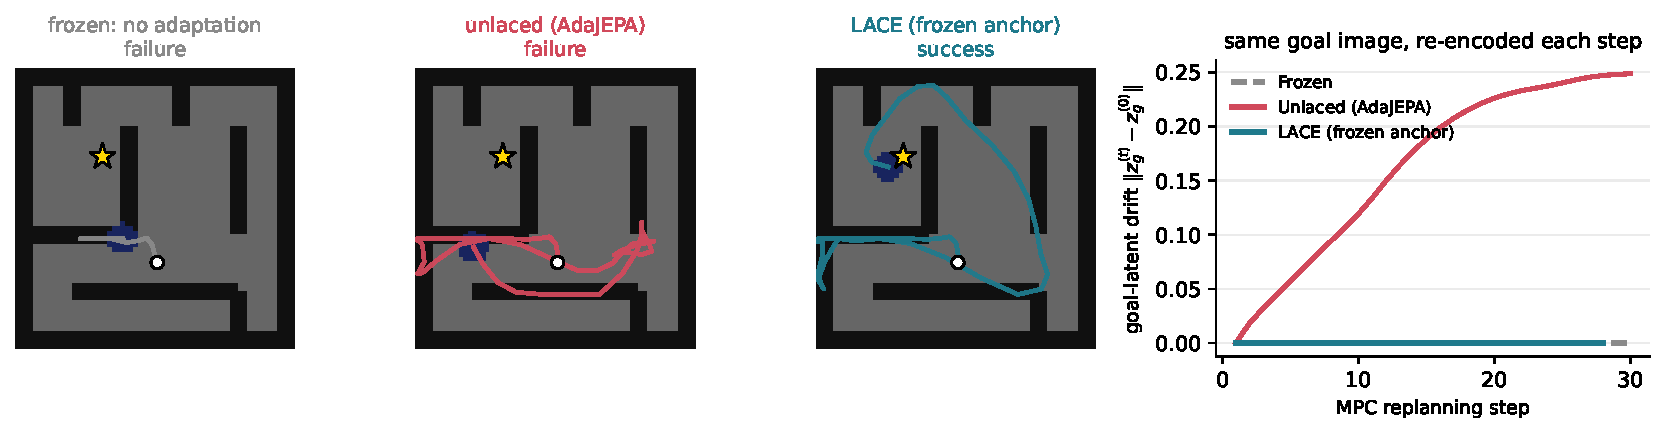
\includegraphics[width=\linewidth]{figures/hook_episode.pdf}
\caption{The failure, in one episode. PointMaze under the dark visual
shift; every arm gets the identical maze, start (white dot), and goal
(star). The frozen model mispredicts and stalls. Self-referential
adaptation (unlaced) reduces its own prediction loss, but re-encoding the
\emph{unchanged} goal image places it somewhere new at every replanning
step (right) --- the planner chases a moving target and fails. Anchored
adaptation (\lace{}) adapts under the same recipe with zero goal drift and
reaches the goal.}
\label{fig:hook}
\end{figure}

Our fix is deliberately minimal. \lace{} (Learning Anchored Consistent
Embeddings) changes one symbol in Equation~\eqref{eq:adajepa}: the target
comes from a \emph{frozen} copy of the pretrained encoder,
%
\begin{equation}
\mathcal{L}_{\lace}
  = \big\| f(\Estud(o_t), a_t) - \Efroz(o_{t+1}) \big\|^2 ,
\label{eq:lace}
\end{equation}
%
(or a slow EMA of the student). The student encoder and predictor may now
adapt at full strength: any relocation of the latent space is penalized
because the target stays put. A corollary falls out for free: the goal should
be encoded by the anchor, pinning the planner's cost landscape to the space
its consumers were calibrated on. Under \lace{}, adaptation may only
re-express the pretrained representation, never invent a new one.

\textbf{Contributions.}
(1)~We identify and name the \emph{head-consistency failure} of
self-referential TTA in latent world models, and make it measurable on public
benchmarks via frozen probe heads (Section~\ref{sec:probes}).
(2)~We propose \lace{}, a one-line anchored-target objective with a
goal-encoding corollary (Section~\ref{sec:method}).
(3)~On miniature reproductions of AdaJEPA's benchmarks (PointMaze shift
suite; a pymunk pusher suite) we show that anchoring costs no planning
success, eliminates goal-latent drift, and survives aggressive symmetric
learning rates that collapse the self-referential objective
(Section~\ref{sec:experiments}).
(4)~On 110 replayed runs (5{,}434 steps) of a deployed screen-interaction
agent, we decompose head damage into an encoder-relocation component that
anchoring removes and a predictor-drift component that it cannot, isolating
each with parameter-subset ablations (Section~\ref{sec:swm}).

\section{Related work}
\label{sec:related}

\textbf{Latent world models and MPC.} World models learned by joint-embedding
predictive architectures (JEPA) \citep{lecun2022path,assran2023ijepa} plan in
latent space without reconstruction \citep{hansen2022tdmpc,zhou2024dinowm}.
Our setting and baseline follow AdaJEPA \citep{anonymous2026adajepa}, which
adapts a JEPA world model online during MPC.

\textbf{Test-time training and adaptation.} TTT with self-supervised
auxiliary tasks \citep{sun2020ttt,gandelsman2022ttt_mae} and entropy
minimization \citep{wang2021tent} adapt perception models at test time; the
collapse risk of self-referential objectives is managed there with restricted
parameter subsets and small steps. The continual-TTA literature has developed
source-anchoring devices against long-horizon drift --- weight-averaged
teachers with stochastic restore \citep{wang2022cotta}, Fisher-weighted
regularization toward source weights \citep{niu2022eata}, self-distillation
from a frozen copy of the source network \citep{song2023ecotta,sata2023} ---
and \citet{zhao2023pitfalls} document that TTA is bounded by the frozen
classifier it feeds. All of this work anchors \emph{classifier logits or
weights} of a perception model under an entropy or pseudo-label objective.
Our setting differs in both loop and objective: the adapted representation
is consumed by an MPC planner and by embedding-space heads, the adaptation
signal is a grounded latent \emph{prediction} loss (a real transition, not a
pseudo-label), and the quantity that must not move is the meaning of the
latent coordinates themselves. We show that in this closed-loop regime the
failure mode is not collapse or forgetting but silent re-mapping ---
invisible to the adaptation loss, fatal to goal embeddings and frozen heads
--- and that anchoring the \emph{prediction target} (rather than logits or
weights) removes it exactly.

\textbf{Stop-gradients, EMA teachers, and collapse.} BYOL and SimSiam avoid
representational collapse with EMA targets and stop-gradients
\citep{grill2020byol,chen2021simsiam}; V-JEPA and TD-MPC2 stabilize latent
prediction similarly \citep{bardes2024vjepa,hansen2024tdmpc2}. \lace{}
transplants this device from \emph{pretraining} (where the teacher and student
co-evolve over millions of steps) to \emph{deployment-time adaptation} (where
the anchor must guarantee consistency with already-calibrated consumers) ---
a different requirement that favors a frozen or very slow anchor
(Section~\ref{sec:e6}).

\textbf{Adaptive control.} Classical adaptive control separates the fixed
reference model from the adapting plant model \citep{astrom2008adaptive};
\lace{} is the representation-learning analogue: the anchor is the reference
frame, the student is the adapting model.

\section{Preliminaries: AdaJEPA}
\label{sec:prelim}

Following \citet{anonymous2026adajepa}: an encoder $z_t = \Estud(o_t)$, an
action encoder $u_t = E_a(a_t)$, and a predictor
$\hat z_{t+1} = f(z_t, u_t)$ are pretrained on reward-free exploration
trajectories with the multi-step latent prediction objective plus
variance/covariance regularization. At test time the agent plans with MPC
(CEM or gradient descent) over the latent rollout cost
$\sum_k \alpha_k \lVert \hat z_{t+k} - z_g \rVert^2$ toward a goal latent
$z_g = \Estud(o_g)$, executes a chunk of actions, and adapts on each observed
transition with Equation~\eqref{eq:adajepa} over a recent-transition buffer,
updating only a parameter subset (by default the last predictor block and the
encoder projection head, with the encoder learning rate $30\times$ smaller).
Weights are episode-local: each episode starts from the pretrained
checkpoint.

\section{The head-consistency failure, and \lace{}}
\label{sec:method}

\subsection{Frozen consumers make the failure visible}
\label{sec:probes}

The adaptation loss of Equation~\eqref{eq:adajepa} is computed \emph{inside}
the adapting representation, so it cannot detect a coordinated re-mapping of
that representation. To measure such re-mapping on public benchmarks we
attach \emph{frozen probe heads}: after pretraining, we freeze the world model
and train small MLPs on its latents --- (i) a success classifier
$p(\text{goal reached} \mid z_t, z_g)$, (ii) a progress regressor estimating
the negative task distance, (iii) a state readout (agent position; block
pose). The probes are then frozen forever. At evaluation, each arm feeds the
probes the latents it actually plans with. A TTA method that merely
re-expresses the pretrained representation keeps probe metrics at
frozen-model levels; one that relocates the space degrades them --- exactly the
quantity a deployed system cares about, since success detectors, safety
monitors, and logging classifiers are all trained offline on the pretrained
space.

\subsection{\lace: anchor the target, anchor the goal}

\begin{figure}[t]
\centering
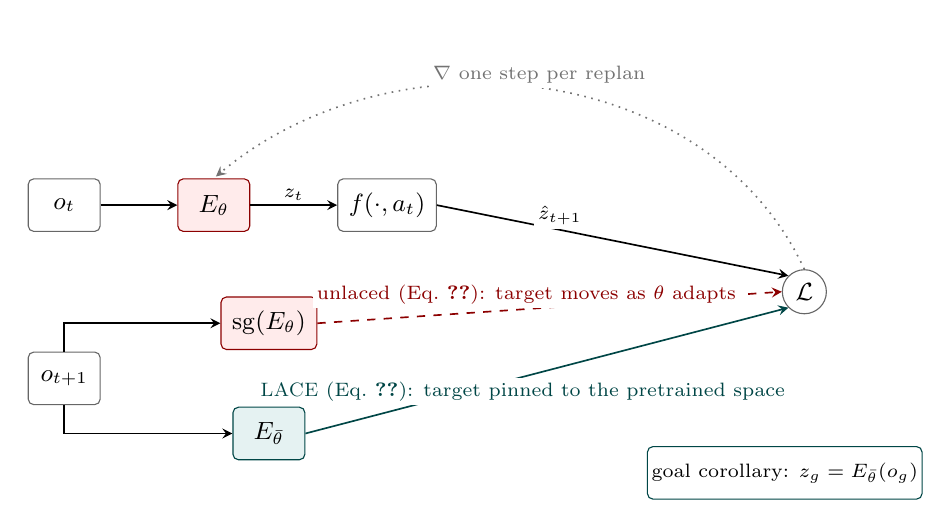
\begin{tikzpicture}[
  font=\small,
  box/.style={draw=black!60, rounded corners=2pt, minimum height=1.9em,
              minimum width=2.6em, inner sep=4pt},
  stud/.style={box, fill=red!8, draw=red!55!black},
  anch/.style={box, fill=teal!10, draw=teal!55!black},
  arr/.style={-stealth, semithick},
  lab/.style={font=\scriptsize, inner sep=1.5pt, fill=white},
]
\node[box] (ot) at (0, 0) {$o_t$};
\node[stud] (enc) at (1.9, 0) {$\Estud$};
\node[box] (f) at (4.1, 0) {$f(\cdot, a_t)$};
\node[draw=black!60, circle, inner sep=2.5pt] (loss) at (9.4, -1.1) {$\mathcal{L}$};
\node[box] (ot1) at (0, -2.2) {$o_{t+1}$};
\node[stud] (senc) at (2.6, -1.5) {$\sg(\Estud)$};
\node[anch] (aenc) at (2.6, -2.9) {$\Efroz$};
\draw[arr] (ot) -- (enc);
\draw[arr] (enc) -- node[lab, above] {$z_t$} (f);
\draw[arr] (f.east) -- node[lab, above, pos=0.35] {$\hat z_{t+1}$} (loss.north west);
\draw[arr] (ot1.north) |- (senc.west);
\draw[arr] (ot1.south) |- (aenc.west);
\draw[arr, red!55!black, dashed] (senc.east) --
  node[lab, above, pos=0.45, text=red!55!black]
  {unlaced (Eq.~\ref{eq:adajepa}): target moves as $\theta$ adapts}
  (loss.west);
\draw[arr, teal!55!black] (aenc.east) --
  node[lab, below, pos=0.45, text=teal!55!black]
  {\lace{} (Eq.~\ref{eq:lace}): target pinned to the pretrained space}
  (loss.south west);
\draw[arr, black!55, dotted, shorten >=1pt] (loss.north) to[out=115,in=40]
  node[lab, above, pos=0.5] {$\nabla$ one step per replan}
  (enc.north);
\node[anch, lab, anchor=west] (goal) at (7.4, -3.4)
  {goal corollary: $z_g = \Efroz(o_g)$};
\end{tikzpicture}
\caption{One TTA step. The prediction branch (top) is shared; the two
objectives differ only in who encodes the target. The self-referential
target (red, dashed) blocks within-step gradients but is re-encoded by the
updated student at every subsequent step, so the loss can still be reduced
by relocating the latent space; the \lace{} anchor (teal) pins the target
--- and, by the same logic, the goal latent --- to the pretrained space.}
\label{fig:method}
\end{figure}

\lace{} replaces the stop-gradient student target with an \emph{anchor}
encoder $\Efroz$ (Figure~\ref{fig:method}):
Equation~\eqref{eq:lace}, where $\bar\theta$ is either (a) the pretrained
encoder weights, frozen (\textbf{laced-frozen}), or (b) a slow EMA
$\bar\theta \leftarrow \tau\bar\theta + (1{-}\tau)\theta$
(\textbf{laced-ema}). The anchor adds one encoder forward per adaptation step
(the target branch already required one) and no planning-time cost.

\emph{Why the stop-gradient is not enough.} AdaJEPA inherits $\sg$ from
SimSiam-style pretraining as an anti-collapse stabilizer
\citep{chen2021simsiam}, and against collapse it works: within one update no
gradient flows through the target, so the loss cannot be reduced by pulling
the target toward the prediction. But the target is re-encoded by the
\emph{updated} student at every subsequent step --- $\sg(\Estud)$ is the
student lagging one update behind, nothing more. Across steps the reference
frame moves freely, and a coordinated relocation of the latent space still
reduces the loss. Consistent with this reading,
\citet{anonymous2026adajepa} report that removing the stop-gradient under
their restricted recipe leaves planning performance similar: it guards
against a failure (collapse) that their conservative recipe already
suppresses, while the failure that matters here (relocation) passes through
it untouched. The stop-gradient buys collapse safety; only the anchor buys a
fixed reference frame.

Two properties follow. \emph{Anchored consistency:} the student can only
reduce the loss by predicting where the \emph{pretrained} encoder will place
the next observation --- modeling dynamics in the fixed reference frame ---
so latent-space relocation is penalized rather than rewarded.
\emph{Goal stability:} since the anchor defines the reference frame, the goal
latent should be computed by it, $z_g = \Efroz(o_g)$. Re-encoding the goal
with the adapting student (the AdaJEPA default) makes the planner chase a
moving target: we measure the drift
$\lVert z_g^{(t)} - z_g^{(0)} \rVert$ directly in Section~\ref{sec:e4}.

The student may learn new dynamics at full learning rate, but the meaning of
the coordinates is inherited, not invented.

\section{Experiments}
\label{sec:experiments}

% Every number in this section is produced from lace/runs/*.json by
% scripts/paper_figs.py and notebooks/lace_paper.ipynb.

We evaluate four arms throughout: \textbf{frozen} (no adaptation),
\textbf{unlaced} (AdaJEPA's self-referential target,
Eq.~\ref{eq:adajepa}), \textbf{laced-frozen} (frozen anchor,
Eq.~\ref{eq:lace}), and \textbf{laced-ema} (EMA anchor, $\tau{=}0.996$).
Unless noted, results use CEM planning, 15 episodes $\times$ 2 seeds per
(shift, arm) cell, and the AdaJEPA adaptation recipe (predictor tail +
encoder head, asymmetric learning rates).

\subsection{Setup: miniature reference benchmarks}
\label{sec:setup}

\textbf{PushObj-mini.} A 2D pusher (velocity-controlled disc) and a rigid
polyomino block on a bounded table (pymunk contact dynamics), rendered to
$64{\times}64$ RGB with a 2-frame history stack. Train shapes
$\{$T, L, Z, $+\}$; held-out test shapes $\{$I, smallT, cube$\}$. Reward-free
pretraining data uses contact-biased Ornstein--Uhlenbeck exploration
(trajectories re-rolled until the block moves; a 30\% pure-OU slice preserves
``no contact, no motion'' examples). Goals are reachable states 8 steps ahead
under the data policy; success requires block pose within 0.5 units and 0.6
rad (modulo each shape's rotational symmetry). Tasks are verified
oracle-solvable (8/8 by ground-truth-state CEM), but the learned world model
plans at $10$--$25\%$ success on this benchmark and the pre-registered
seen-vs-unseen generalization gate did not pass (gap $2.2$\,pp, threshold
$10$\,pp); we therefore use PushObj for the drift and anchor-speed analyses
(E4, E6), where its longer horizons are informative, and do not rest planning
claims on it.

\textbf{PointMaze-mini.} A point mass in procedurally generated mazes with
dynamics shifts (mass $\times 0.2$, damping $\times 8$), visual corruptions
(blur, salt-and-pepper, darkening, agent recolor), and held-out layouts.

Both use the same small CNN encoder (128-d latent), residual-MLP predictor,
CEM/GD planners, and the AdaJEPA adaptation recipe. Pre-registered pass/fail
gates for every claim were committed before the grid ran
(\texttt{GATES.md} in the code release).

\subsection{E1: adaptation gains transfer across target sources}
\label{sec:e1}

\begin{figure}[t]
\centering
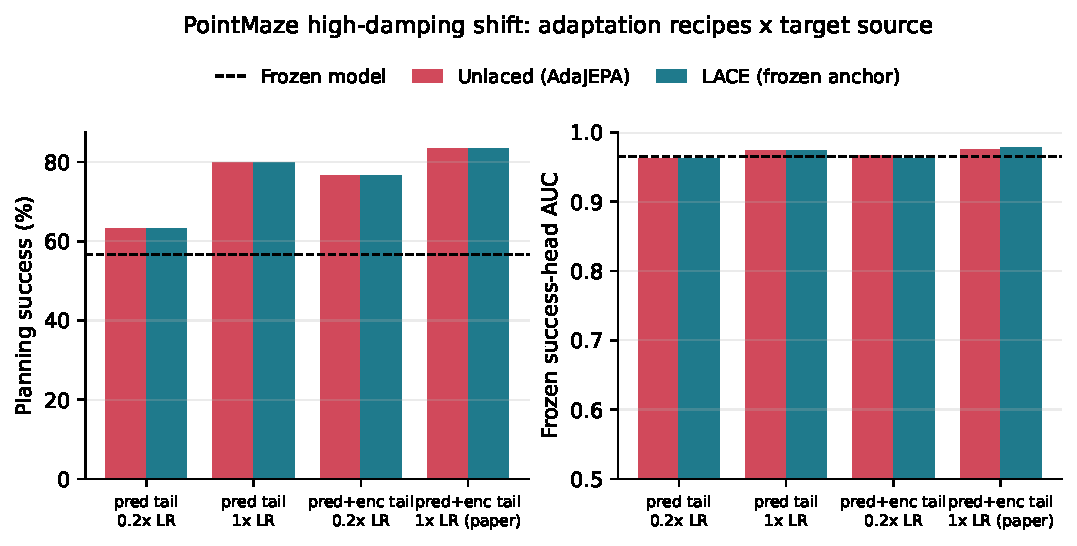
\includegraphics[width=\linewidth]{figures/e1_maze_grid.pdf}
\caption{PointMaze high-damping shift, four adaptation recipes $\times$ two
target sources. Anchoring the target costs nothing: laced (teal) matches
unlaced (red) planning success at every recipe (left), and within short
episodes at conservative rates neither damages the frozen success head
(right). The damage appears under pressure --- Sections~\ref{sec:e3},
\ref{sec:e4}, and \ref{sec:swm}.}
\label{fig:e1}
\end{figure}

On the high-damping maze shift, adaptation lifts planning success from
$56.7\%$ (frozen) to $83.3\%$ with the full recipe, and the lift is
\emph{identical} whether the target is the student or the frozen anchor
(Figure~\ref{fig:e1}, left): anchored consistency does not tax adaptation.
Probe AUC stays near the frozen level ($0.96$--$0.98$) for all arms --- with
the paper's conservative asymmetric learning rates and short episodes, the
maze alone does not expose the failure. Three stressors do: goal-latent
drift (E4), symmetric learning rates (E3), and long-horizon deployment (E7).

\subsection{E2: full shift suites}
\label{sec:e2}

\begin{figure}[t]
\centering
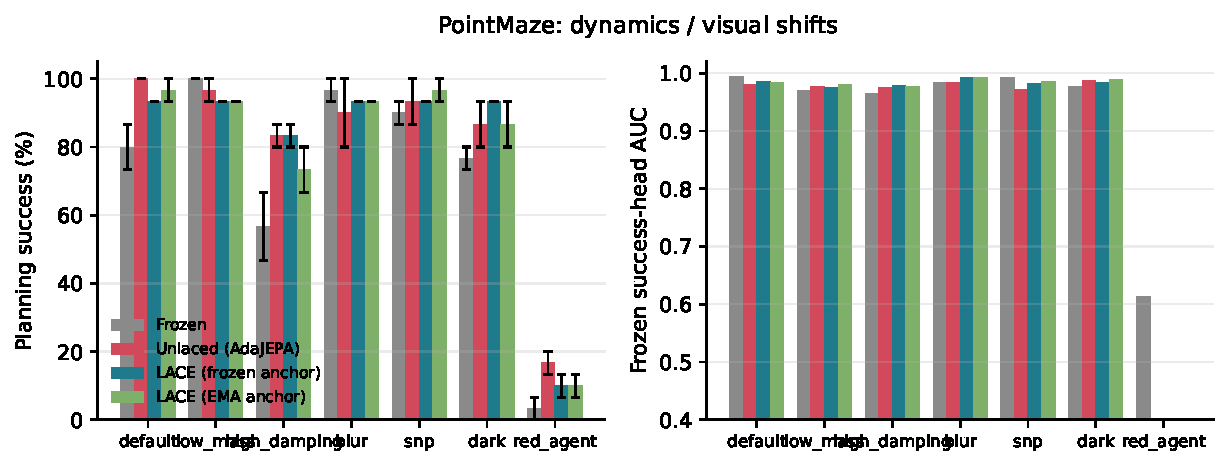
\includegraphics[width=\linewidth]{figures/e2_maze_shifts.pdf}
\caption{PointMaze shift suite (dynamics + visual), all four arms.}
\label{fig:e2maze}
\end{figure}

Across the maze suite (Figure~\ref{fig:e2maze}), the laced arms match or
beat unlaced planning success in aggregate --- dynamics: laced-frozen
$88.3\%$ vs unlaced $90.0\%$ (frozen $78.3\%$); visual: $72.5\%$ vs
$71.7\%$; held-out layouts: laced-ema $44.4\%$ vs unlaced $45.6\%$ (frozen
$35.6\%$). With the gradient-descent planner on dynamics shifts the
anchored arm is strongest ($90.0\%$ vs $70.0\%$ unlaced): GD planning is
more sensitive to the smoothness of the cost landscape, which the anchor
preserves. On PushObj-mini the planner operates near its noise floor
(Section~\ref{sec:setup}), so per-arm differences are within error bars; we
report the suite for completeness and lean on the maze and deployment data
for the planning claims.

\subsection{E3: symmetric learning rates and collapse safety}
\label{sec:e3}

\begin{figure}[t]
\centering
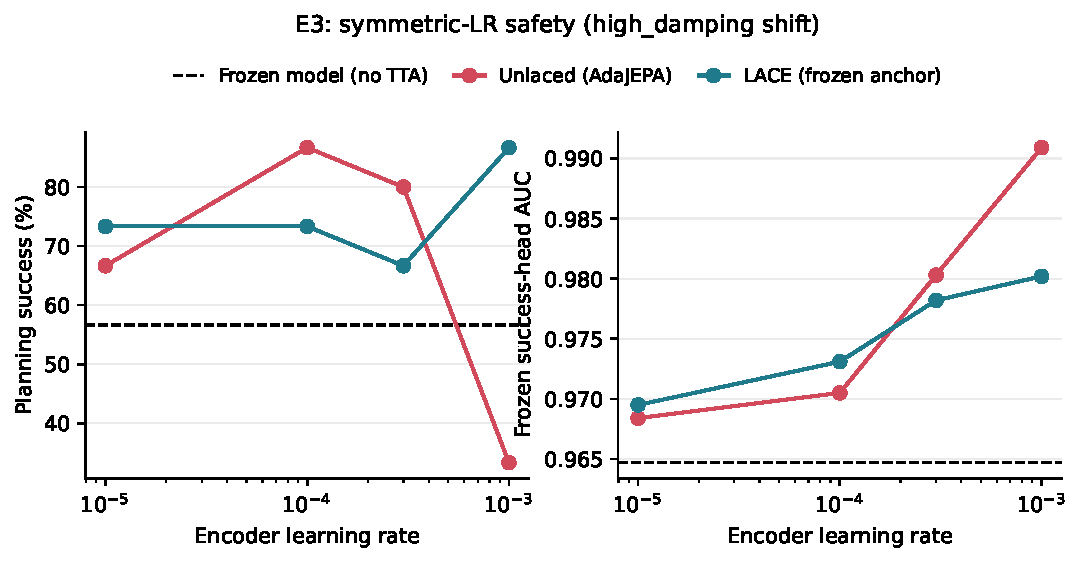
\includegraphics[width=\linewidth]{figures/e3_lr_sweep.pdf}
\caption{Symmetric-LR sweep on the high-damping shift; dashed line marks
the frozen (no-TTA) baseline. At $\eta_{\text{enc}}{=}10^{-3}$ the
self-referential target collapses planning ($33.3\%$, below frozen) while
the anchored target keeps improving ($86.7\%$).}
\label{fig:e3}
\end{figure}

AdaJEPA adapts the encoder $30\times$ slower than the predictor; this
asymmetry is the standard defense against self-referential drift. E3 removes
it: encoder and predictor share one learning rate, swept over
$\{10^{-5}, 10^{-4}, 3{\times}10^{-4}, 10^{-3}\}$. The unlaced arm improves
until $3{\times}10^{-4}$ and then collapses at $10^{-3}$ ($33.3\%$ success,
worse than never adapting). The laced arm is monotone in the sweep and
\emph{best} at the most aggressive rate ($86.7\%$): with the target pinned,
a larger step size only means faster convergence to the anchored solution,
not faster relocation. Anchoring replaces a fragile hyperparameter with a
structural guarantee.

\subsection{E4: goal-latent drift}
\label{sec:e4}

\begin{figure}[t]
\centering
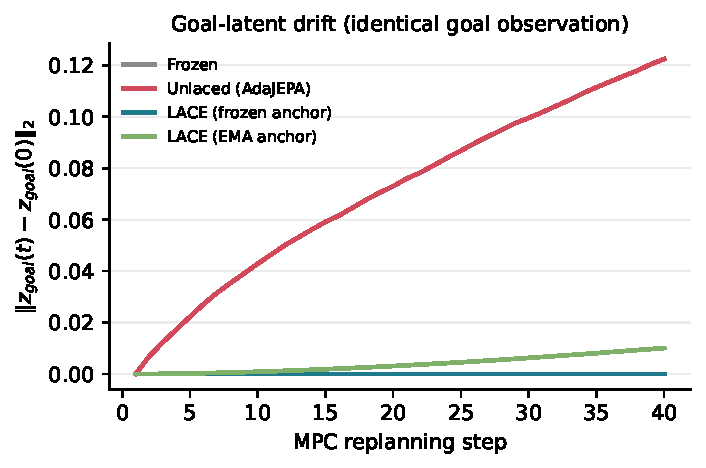
\includegraphics[width=0.62\linewidth]{figures/e4_goal_drift.pdf}
\caption{Goal-latent drift $\lVert z_g^{(t)} - z_g^{(0)}\rVert$ pooled over
the PushObj suite. The goal observation never changes; any drift is encoder
relocation.}
\label{fig:e4}
\end{figure}

The cleanest signature of relocation needs no probes: re-encode the
\emph{same} goal observation at every replanning step and measure how far
its latent moves. Unlaced drifts steadily (mean final drift $0.11$ on
PushObj, $0.21$ on the maze suite --- roughly $8\%$ of the typical
inter-state latent distance); laced-frozen is exactly zero by construction,
and laced-ema stays two orders of magnitude smaller ($0.008$). The planner
in the unlaced arm is chasing a target that moves because the map, not the
territory, is changing.

\subsection{E5: low-data pretraining}
\label{sec:e5}

\begin{figure}[t]
\centering
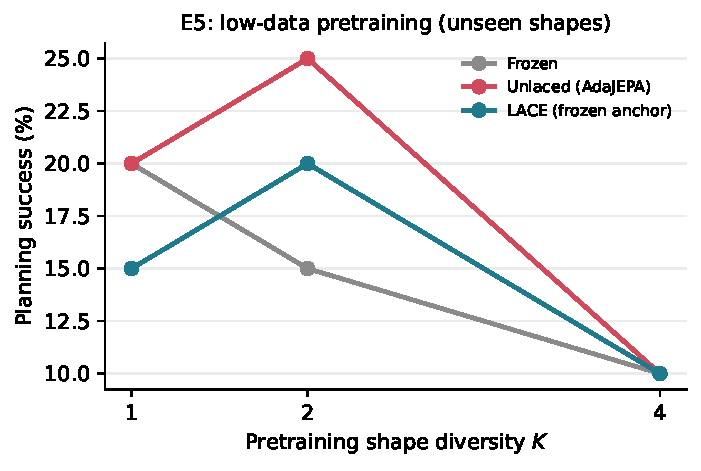
\includegraphics[width=0.58\linewidth]{figures/e5_lowdata.pdf}
\caption{Planning success on unseen PushObj shapes vs pretraining shape
diversity $K$. Adaptation helps most where data is scarcest, and the
anchored target keeps pace with the self-referential one.}
\label{fig:e5}
\end{figure}

Sweeping pretraining shape diversity $K \in \{1,2,4\}$ on PushObj and
evaluating on unseen shapes (Figure~\ref{fig:e5}), adaptation helps most
exactly where data is scarcest --- both targets lift $K{=}1,2$ success,
consistent with AdaJEPA's data-compensation result, and are again
indistinguishable. Probe AUC in this regime is dominated by the pretrained
representation itself (frozen-arm AUC falls from $0.96$ at $K{=}4$ to $0.67$
at $K{=}1$), so head-consistency comparisons at $K{=}1$ mostly measure the
probes' failure to fit, not adaptation damage --- a limit of the probe
methodology at very low data.

\subsection{E6: how slow must the anchor be?}
\label{sec:e6}

\begin{figure}[t]
\centering
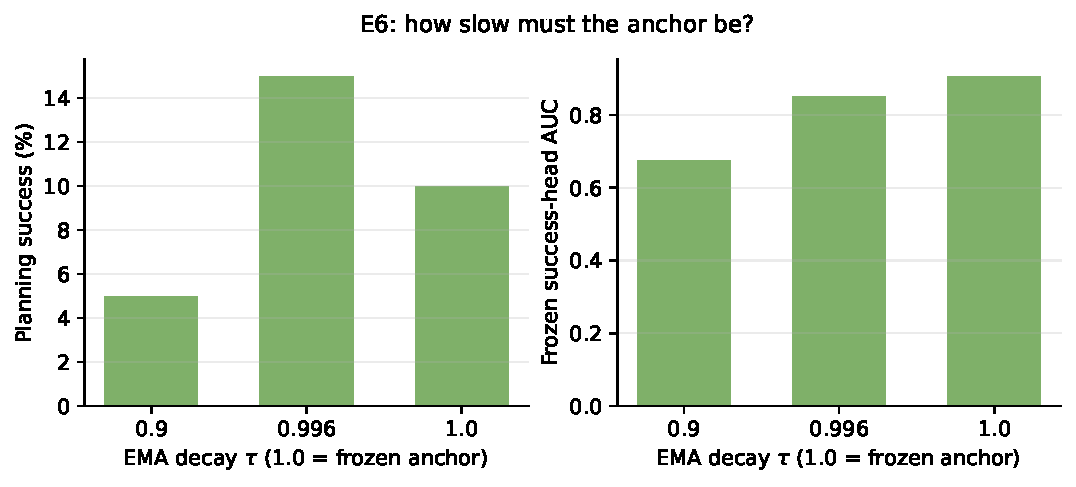
\includegraphics[width=\linewidth]{figures/e6_ema_decay.pdf}
\caption{EMA-decay sweep on unseen PushObj shapes. A fast anchor
($\tau{=}0.9$) is self-reference in slow motion; $\tau{=}0.996$ and the
frozen anchor ($\tau{=}1.0$) preserve both planning success and head
consistency.}
\label{fig:e6}
\end{figure}

Sweeping the EMA decay $\tau \in \{0.9, 0.996, 1.0\}$ on unseen PushObj
shapes (Figure~\ref{fig:e6}): a fast anchor ($\tau{=}0.9$) is
self-reference in slow motion --- probe AUC falls to $0.68$ and planning
success to $5\%$ --- while $\tau{=}0.996$ and the frozen anchor hold AUC at
$0.85$--$0.91$. The anchor must move at most negligibly over the horizon on
which downstream consumers were calibrated; when in doubt, freeze it.

\subsection{E7: deployed screen-interaction agent}
\label{sec:swm}

\begin{figure}[t]
\centering
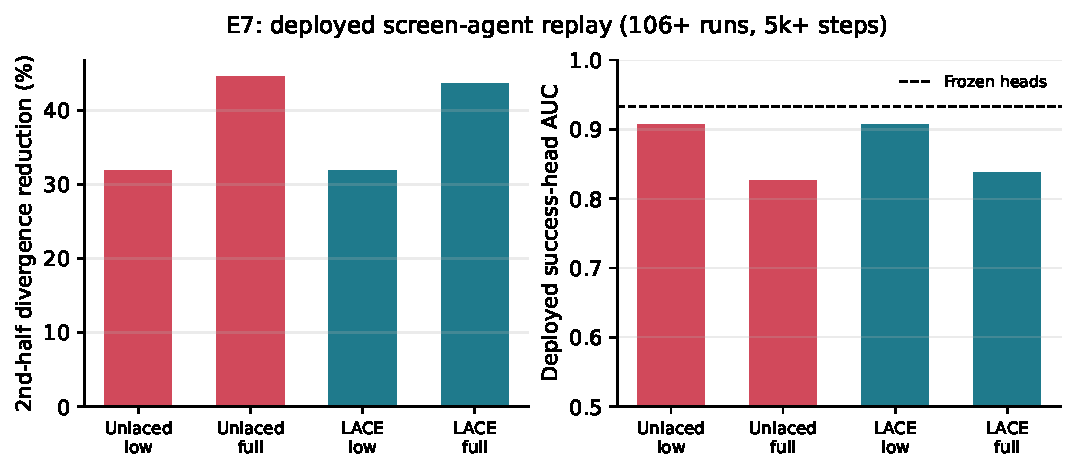
\includegraphics[width=\linewidth]{figures/e7_swm_replay.pdf}
\caption{Prequential replay of 110 deployed runs (5{,}434 steps): each
transition is scored before being adapted on. Divergence gains (left)
survive anchoring; deployed-head AUC (right) recovers only partially,
motivating the mechanism decomposition (Figure~\ref{fig:e7b}).}
\label{fig:e7}
\end{figure}

\begin{figure}[t]
\centering
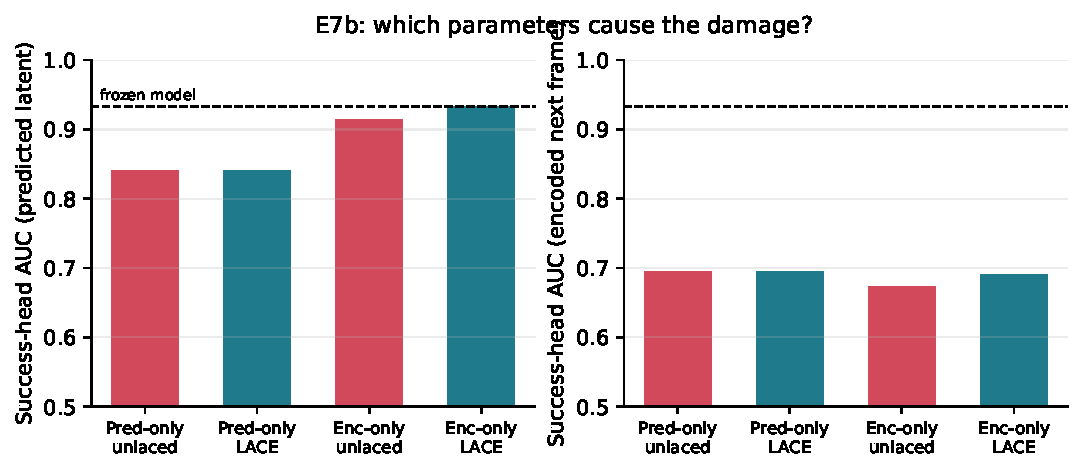
\includegraphics[width=\linewidth]{figures/e7b_mechanism.pdf}
\caption{Parameter-subset ablation on the replay. Adapting only the
predictor already reproduces most of the pred-latent AUC damage, and
anchoring cannot prevent it (the anchor constrains the \emph{target}, not
predictor overfitting to the small transition buffer). Encoder-space AUC
(right) isolates the relocation component that anchoring does remove.}
\label{fig:e7b}
\end{figure}

The deployment replay is where the phenomenon was first observed, and it is
also where the simple story breaks --- we report both halves. On 110
recorded runs of a screen-interaction agent (5{,}434 transitions,
prequential scoring: each step is evaluated before the model adapts on it),
the published full recipe cuts second-half prediction divergence by
$44.6\%$ while the deployed success head's AUC on predicted latents falls
from $0.933$ to $0.826$. Anchoring the target recovers only a fraction
($0.838$) --- our pre-registered gate for this experiment
(AUC within $0.02$ of frozen) \emph{fails}.

The parameter-subset decomposition (Figure~\ref{fig:e7b}) explains why.
Head damage here has two mechanisms: (i)~\emph{encoder relocation}, the
self-reference failure this paper is about, which anchoring removes
completely --- adapting only the encoder with the self-referential target
drops pred-latent AUC to $0.914$ and encoder-space AUC below baseline
($0.674$ vs $0.695$), while the same adaptation with an anchored target
restores both exactly to frozen levels ($0.933$, $0.691$); and
(ii)~\emph{predictor drift} --- adapting only the predictor drops AUC to
$0.840$ \emph{identically} under both target sources, because the anchor
constrains the target, not the predictor's overfitting to the small
recent-transition buffer. \lace{} is therefore necessary but not sufficient
at deployment scale: it solves the representation half of the problem
exactly, and sharply exposes the optimization half (buffer size, step count,
trust regions on the predictor), which we leave open.

\section{Discussion and limitations}
\label{sec:discussion}

\textbf{The anchor-drift tension.} A frozen anchor guarantees consistency but
can never incorporate a truly novel world; under persistent shift the anchored
target is eventually wrong about \emph{content}, not just coordinates. The EMA
anchor trades consistency for plasticity (E6); scheduling that trade --- and
re-calibrating consumers when the anchor must move --- is the continual
learning question this paper deliberately does not solve.

\textbf{Scale.} Our benchmarks are miniature by design (minutes per training
run on a laptop GPU); the deployment replay is the evidence that the
phenomenon and the fix survive contact with reality. Scaling LACE to
foundation-scale world models is future work.

\textbf{When unlaced TTA is fine.} If nothing downstream is frozen --- no
fixed goal embeddings, no calibrated heads, single-episode tasks scored only
by environment reward --- self-referential TTA's extra freedom can be harmless
at conservative learning rates (our maze grids show small recipes cause little
damage within short episodes). The failure grows with adaptation pressure:
step count, learning rate, and encoder participation.

\section*{Reproducibility statement}
All environments, training, adaptation, evaluation, probes, and figures are
released with exact seeds and one-command reproduction scripts at
\url{https://github.com/bourkefloyd/lace-tta}. The
deployment replay data is proprietary telemetry and is not released; we
report aggregate metrics only, and the public benchmarks reproduce the
phenomenon end-to-end.

\section*{Acknowledgments}
We thank the AdaJEPA authors for a reproducible and clearly written method.

\bibliographystyle{plainnat}
\bibliography{refs}

\end{document}
